%!TEX root=../Vorlage_DA.tex
%	########################################################
% 				Git
%	########################################################


%	--------------------------------------------------------
% 	Allgmeine Hinweise
%	--------------------------------------------------------
\section{Git}

Git\footnote{\url{https://de.wikipedia.org/wiki/Git}} ist eine dezentrales Versionsverwaltungssystem\footnote{\url{https://de.wikipedia.org/wiki/Versionsverwaltung}} welches urspr\"unglich f\"ur die Entwicklung des Linux-Kernels entwickelt wurde. Es geh\"ort zu den meistgenutzten Systemen in der OpenSource Softwareentwicklung, da es gegen\"uber zentralen Versionsverwaltungssystemen diverse Vorteile besitzt:

\begin{itemize}
  \item kein zentraler Server notwendig
  \subitem Versionshistory ist lokal verf\"ugbar
  \subitem Alle Operationen sind lokal
  \item Kryptographische Sicherheit der Projektgeschichte
  \item Gute Performance
\end{itemize}

Nachteilig ist, dass es zu Merge-Konflikten kommen kann, wenn mehrere Personen die gleiche Datei ver\"andert haben, und diese von Git nicht automatisch miteinander Verschmolzen werden kann. In diesem Fall muss dies manuell durchgef\"uhrt werden. Bei einer Zentralen Versionsverwaltung w\"are dies nicht m\"oglich, da dort nur jeweils 1. Person pro Datei arbeiten darf.

Wir haben uns f\"ur Git entschieden, da wir einerseits durch die Dezentralit\"at gleichzeitig, auch ohne Internetverbindung an dem Projekt arbeiten k\"onnen. Des Weiteren wird uns die M\"oglichkeit gegeben Quellcode\"anderungen mehrerer Personen zu Mergen, sobald eine Funktion ausreichend stabil ist.

\subsection{Grundlegende Funktionsweise}

Bei git besitzt jeder Programmierer ein eigenes Repository, auf welchem er \"anderen commitet. Diese k\"onnen dann gesammelt auf einen Zentrales Repository geladen werden, welches dann den aktuellen Projektstand repr\"asentiert.

Wenn ein aktueller Projektstand in das eigene Repository eingecheckt wird, nennt man dies einen Commit. Dieser umfasst die ge\"anderten Dateien, wie auch einen Text welcher die \"Anderungen repr\"asentiert.

\begin{figure}[h]
\centering
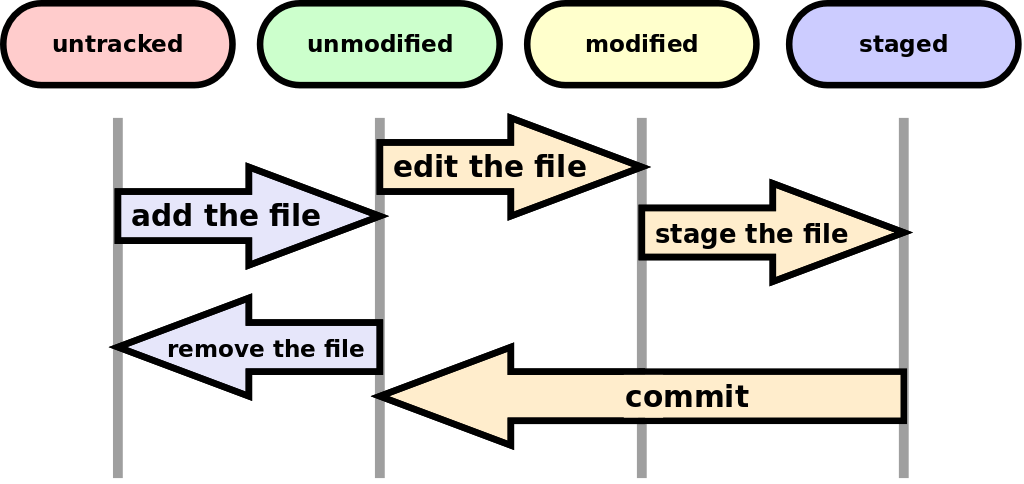
\includegraphics[width=0.9\textwidth]{./media/images/development/git_file_status_livecycle.png}
\caption{grundlegender Zyklus, in der sich der Dateistatus laufend \"andert}
\label{git_file_status_livecycle}
\end{figure}


\htlParagraph{Vormerken aller ge\"anderten Dateien}

\begin{lstlisting}[language=bash]
git add -u
\end{lstlisting}

\htlParagraph{Einchecken  aller Vorgemerkten Dateien}

\begin{lstlisting}[language=bash]
git commit -m 'this is my first commit'
\end{lstlisting}

\section{GitHub}

GitHub\footnote{\url{https://github.com}} ist eine der am weitesten verbreitetsten Hosting-Dienst welcher in der Open-Source Software Entwicklung genutzt wird. Als grundlegende Versionsverwaltung wird git genutzt, welches mithilfe der Webbasierten Oberfl\"ache von GitHub einfach verwaltet wird.

\subsection{Grundlegender Arbeitszyklus}

Wir haben uns auf ein grundlegendes Arbeitsverfahren geeinigt, welches sicherstellt das das Projekt m\"oglichst fehlerfrei verwaltet werden kann. Dazu hat jedes Projektmitglied einen fork des Projektes auf seinem eigenen GitHub-Repository, mithilfe dessen er dann Pull-Requests an das zentrale Repository stellen kann.

Vorteile dieses Verfahrens sind unter anderem, dass das Mergen im Normalfall auf dem Server geschieht. Desweiteren wird jedes Pull-Request automatisch getestet, und wird erst nach einem erfolgreichem Test in das zentrale Repository eingecheckt. So werden auftretende Probleme wie fehlende Dateien oder Inkompatibilit\"aten mit anderen \"Anderungen besonders schnell gefunden.